\documentclass{article}


\usepackage{arxiv}

\usepackage[utf8]{inputenc} % allow utf-8 input
\usepackage[T1]{fontenc}    % use 8-bit T1 fonts
\usepackage{hyperref}       % hyperlinks
\usepackage{url}            % simple URL typesetting
\usepackage{booktabs}       % professional-quality tables
\usepackage{amsfonts}       % blackboard math symbols
\usepackage{nicefrac}       % compact symbols for 1/2, etc.
\usepackage{microtype}      % microtypography
\usepackage{lipsum}
\usepackage{fancyhdr}       % header
\usepackage{graphicx}       % graphics
\graphicspath{{figures/}}     % organize your images and other figures under figures/ folder

\usepackage{amsmath,amsfonts,amssymb,amsthm,mathtools,esint,eucal}  %math
\usepackage{subcaption}
%Header
\pagestyle{fancy}
\thispagestyle{empty}
\rhead{ \textit{ }} 

% Update your Headers here
\fancyhead[LO]{Running Title for Header}
% \fancyhead[RE]{Firstauthor and Secondauthor} % Firstauthor et al. if more than 2 - must use \documentclass[twoside]{article}
  
%% Title
\title{Generating Synthetic Data via Intent-Preserving and Intent-Corrupting Augmentations for Multi-task Training Dialogue Embeddings.
%%%% Cite as
%%%% Update your official citation here when published 
\thanks{\textit{\underline{Citation}}: 
\textbf{Authors. Title. Pages.... DOI:000000/11111.}} 
}

\author{
  Ilya Alekseev \\
  Neural Networks and Deep Learning Lab \\
  Moscow Institute of Physics and Technology \\
  \texttt{ilya\_alekseev\_2016@list.ru} \\
  %% examples of more authors
   \And
  Denis Kuznetsov \\
  Neural Networks and Deep Learning Lab \\
  Moscow Institute of Physics and Technology \\
  \texttt{kuznetsov.dp@phystech.edu} \\
  %% \AND
  %% Coauthor \\
  %% Affiliation \\
  %% Address \\
  %% \texttt{email} \\
  %% \And
  %% Coauthor \\
  %% Affiliation \\
  %% Address \\
  %% \texttt{email} \\
  %% \And
  %% Coauthor \\
  %% Affiliation \\
  %% Address \\
  %% \texttt{email} \\
}


\begin{document}
\maketitle


\begin{abstract}
Text embeddings from pre-trained language models have been proven to be extraordinarily useful for various sentence-level tasks, such as pair classification, similarity estimation, and retrieval. Corresponding models are usually trained on large amounts of clean and diverse data using contrastive loss. Unfortunately, there are no such datasets for the domain of dialogue data. In this work, we describe the process of mining a synthetic dataset of dialogues for contrastive learning with hard negatives. We investigate various augmentation strategies for constructing dialogues with preserved or corrupted intents (positive and negative samples, respectively). To demonstrate the stated cleanliness and diversity, we train a dialogue encoder model and analyze its properties.
\end{abstract}


% keywords can be removed
\keywords{text embedding \and dialogue \and synthetic data \and augmentation \and natural language processing}


\section{Introduction}
Obtaining embeddings is one of the key tasks in machine learning and popular one in recent years. Vector representation of an object is a convenient mathematical object. If an embedding accurately and comprehensively encodes the semantics of the original data, it opens up the possibility of using it in a wide range of tasks.

In the field of natural language processing, classical methods for text vectorization such as bag of words \cite{bow} and tf-idf \cite{SprckJones2021ASI} have long been discovered. Thanks to deep learning, we have witnessed remarkable word vectorizations such as word2vec \cite{mikolov2013efficient} and GloVe \cite{pennington-etal-2014-glove}, which convey the semantic similarity between words; CoVe \cite{mccann2018learned} and ELMo \cite{peters-etal-2018-deep}, which encode information about the surrounding context. Recently, powerful encoder models have emerged that produce general-purpose text embeddings \cite{xiao2023cpack, wang2022text, li2023general}. They incorporate so much semantic information about texts that it can be applied to tasks such as classification, clustering, ranking, semantic textual similarity, and more. The success of these models is largely attributed to the use of contrastive learning on massive datasets. 

However, the more specific the data structure, the more challenging it is to mine a large dataset. As of today, there are no encoding methods for entire dialogues. In other words, there is no way to obtain a dense vector representation that conveys universal information about a dialogue. There are language models that adapt successfully to the hierarchical and temporal nature of dialogue \cite{zhang-etal-2023-dialog, li2022future}, but they only address tasks at the token and utterance levels, not at the dialogue level. There are text encoders for utterances in a dialogue \cite{henderson2020convert, Zhou2022}, but not for the entire dialogue.

Data is almost always scarce when it comes to building dialogue models. To date, numerous methods for generating synthetic dialogues have been devised \cite{kim2021neuralwoz, mohapatra2021simulated, wan-etal-2022-unified, zheng2023augesc}, but they do not generate dialogues in pairs \cite{schick2021generating}, as is conceptually important for contrastive learning. The simplest way to expand a training dataset is through augmentation \cite{soudani2023data}. However, we find them insufficient, as they do not significantly alter the structure of the dialogue. In this work, we will describe a method for constructing a synthetic dataset of dialogue pairs using various augmentations that preserve or alter the set of intents in the dialogue. These augmentations can be used for contrastive learning together with other tasks for pretraining powerful dialogue embeddings.

\section{Problem Formulation}

\textbf{Dialogue Data.} A dialogue is defined as the following list:
$$
d=[(u_1, s_1), \ldots, (u_n, s_n)],
$$
where $u_i$ represents the utterance of a participant in the dialogue at step $s_i$. We are interested in so-called task-specific dialogues with two participants: the system and the user. With some approximation, they can be described as dialogues between a customer and a service worker (or a robot). During the dialogue, the customer has various intents that the worker strives to fulfill. These intents can be finding a restaurant and booking a table, calling a taxi, or purchasing a train ticket. We will consider two dialogues similar if they have a similar set of intents.

\textbf{Augmentation.} By augmentation, we mean the generation of new valid examples by transforming existing ones. Valid examples are those that sufficiently resemble real-world data. Let $D$ be the set of valid objects. Then augmentation is a non-identical mapping $\text{aug}(d)$ that does not take objects outside the set of valid objects:
$$
\text{aug}: D\to D.
$$
Typically, this generation is implemented by making small changes to a valid training object. For example, image augmentation might involve slight rotations or blurring. Text augmentation is especially challenging because validity implies adherence to language rules, meaningfulness and a certain style. In the case of dialogues, it is necessary to maintain the structure and role differentiation, as indicated earlier.

\textbf{Embedding.} Embedding is a mapping of $D$ to a vector space:
$$
e:D\to E\subseteq\mathbb{R}^d.
$$
For an object $d$, its embedding $e(d)$ should convey some semantics of $d$. This is reflected in the fact that $e(d)$ may contain lexical information or latent features useful for classification and other downstream tasks. It is especially valuable if using embeddings $e(a), e(b)$ allows for assessing the semantic similarity of objects $a, b$.

\section{Related Works}

\texttt{this section is incomple, this is still a draft }

AugSBERT \cite{thakur2021augmented} can be viewed as the similar approach to ours one, but their augmentation uses an already presented dataset of text pairs, which is absent in our case.

\section{Approach}

\subsection{Augmentations} \label{sec:aug}

\textbf{Token Insertion.} One of the simple yet effective ways to augment text is to lengthen it by inserting extra tokens. For this purpose, we added a special token `<mask>` to random places in the dialogues and used transformer models trained on the MLM task to fill these masks \cite{devlin2019bert}. Insertion is rejected if the token proposed by the model is only a fragment of a word \cite{wu2016googles, sennrich-etal-2016-neural} or if the prediction probability is below a manually set threshold. To take the dialogue context into account during token insertion, multiple consecutive responses were fed into the mask-filling model at once as a compromise between feeding single utterances and entire dialogue.

\textbf{Token Replacement.} This method is identical to the previous one, except that instead of adding the `<mask>` token, some tokens in the original dialogue are replaced. In this case, the mask-filling model is fed with single utterances to make replacements more diverse and random.

\textbf{Back Translation.} Translation from the original language to another language and then back to the original language. Neural machine translation models were used for this purpose \cite{TiedemannThottingal}.

\textbf{Shuffling Utterances.} Previous augmentations modify the dialogue within a single utterance, since they are methods applicable to arbitrary text data. It seems essential to learn how to change the order of utterances in a dialogue to create new valid dialogue. For this purpose, we propose using a model that measures the similarity between utterances within a dialogue. Using these similarities, it is possible to cluster utterances within each dialogue. Experiments showed that these clusters represent significant individual stages of the dialogue that can be shuffled with each other.

\textbf{Shortening Dialogue.} Individual clusters of utterances within the dialogue can be discarded, resulting in a pruned dialogue with fewer utterances.

\textbf{Lengthening Dialogue.} The special model was trained to arrange a list of given utterances. This transformer takes the text embeddings of each utterance as input sequence, without specifying information about their order in the original dialogue. It outputs ranks that can be used to "sort" the utterances to restore the original order. If some external responses are added to the original dialogue, this model generates a new, longer dialogue.

The augmentations mentioned above can be configured to either preserve or alter intent. Specifically, token replacement can be viewed as intent-corrupting augmentation, because all the keywords such as "restaurant", "taxi" etc. tend to be replaced. Pruning dialogue may remove some intents, but the result is still much similar to original dialogue, since its intents are fully encompassed by the original dialogue's intents. 
Shuffling utterances doesn't change any intents, it only changes their order. The rest of augmentations preserves intents because they either perform paraphrasing (back translation), or add new information (token insertion, lengthening dialogue).

To expand the set of augmentations even further, we use a composition of several. More details about augmentation implementations are presented in appendix.

\subsection{Dialogue Encoder Architecture}

As a baseline method for vectorization, we use RoBERTa \cite{liu2019roberta} without any modifications. The input is \texttt{[CLS] ut1 [SEP] ut2 [SEP] ut3 [SEP]}, and the output is the hidden state of \texttt{[CLS]} token from the last layer. 

For a slightly advanced dialogue language model, we use HSSA \cite{zhang-etal-2023-dialog}. It uses BERT \cite{devlin2019bert} as a backbone and modifies its attention to capture the hierarchical structure of dialogue and reach the computational trade-off between feeding a transformer separate utterances and feeding an entire dialogue.

\subsection{Pre-train Tasks}

To make the encoder produce rich vector representations, it is necessary to train it to perform tasks where semantic features are engaged. A popular task is contrastive learning:
$$
\mathcal{L}=-\log{\exp(\text{sim}(x,y))\over\sum_{z}\exp(\text{sim}(x,z))}.
$$
Here, $x=e_\theta(a), y=e_\theta(b)$ are embeddings of a pair of semantically similar objects and $z=e_\theta(c)$ is semantically distant from $x$, $\text{sim}$ is a metric similarity function. This task trains embeddings to convey semantic similarity as metric similarity.

\section*{Acknowledgments}
This was was supported in part by......

%Bibliography
\bibliographystyle{unsrt}  
\bibliography{references}  

\appendix
\section{Dialogue Dataset}
Large dataset is important for contrastive learning. For training our models, we took a merge of some task-oriented datasets from DialogStudio collection \cite{zhang2023dialogstudio}. All of them are listed in the table \ref{tab:dataset}.

\begin{table}[!htb]
    \centering
    \begin{tabular}{c|c|c|c}
        Name & \# dialogues & \# utterances & \# tokens \\
        \hline
        AirDialogue & 321K & 4086K & 49.4M \\
        SimJointGEN & 100K & 1584K & 22.5M \\
        MS-DC & & & \\
        MetaLWOZ & & & \\
        MULTIWOZ2\_2 & & & \\
        SGD & & & \\
        KETOD & & & \\
        FRAMES & & & \\
        Disambiguation & & & \\
        ABCD & & & \\
        AirDialogue & & & \\
        BiTOD & & & \\
        Taskmaster1 & & & \\
        \textbf{Total} & & & \\
        \textbf{Filtered} & 501K & 6320K & 83.7M
    \end{tabular}
    \caption{All the datasets are taken from DialogStudio collection \cite{zhang2023dialogstudio}}
    \label{tab:dataset}
\end{table}

\section{Auxiliary Models} \label{app:aug}

As mentioned in Section \ref{sec:aug}, we trained special models to perform dialogue-level augmentations.

\begin{figure}[!htb]
    \centering
    \begin{subfigure}[t]{0.6\linewidth}
        \centering
        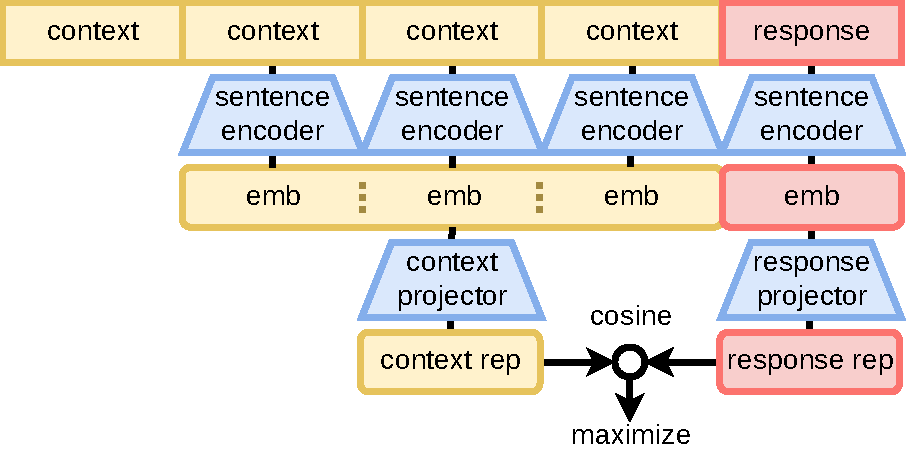
\includegraphics[width=0.9\linewidth]{figures/pairwise.drawio.pdf}
        \caption{for measuring similarities between utterances}
        \label{fig:pairwise}
    \end{subfigure}
    \begin{subfigure}[t]{0.35\linewidth}
        \centering
        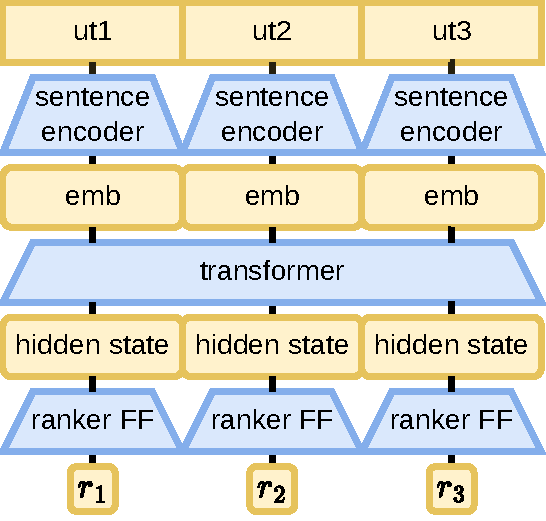
\includegraphics[width=0.9\linewidth]{figures/listwise.drawio.pdf}
        \caption{for lengthening dialogue}
        \label{fig:listwise}
    \end{subfigure}
    \caption{Auxiliary models for performing augmentations.}
    \label{fig:enter-label}
\end{figure}

\subsection{Pairwise Model}

We utilized a model for measuring the similarity between dialog utterances. In its basic form, it can be implemented as follows: take sentence embeddings of the utterances and compare the cosine similarities between them. Training such a model on sequential utterances using contrastive learning yields commendable utterance embeddings \cite{Zhou2022}.

However, this approach has a significant drawback; it does not consider the context from several preceding utterances. In a dialogue, it is crucial to compare not just pairs of utterances but pairs of context-response. Therefore, we employed the following model (fig. \ref{fig:pairwise}):

\begin{enumerate}
    \item  First, embeddings for all context utterances $c=[u_1,\ldots,u_k]$ and the response $r$ are obtained using a pretrained sentence encoder.
    \item The embeddings of the context are concatenated and passed to a projector that outputs a vector representing the context.
    \item The response embedding is fed into a second encoder, resulting in a vector representing the response.
    \item The cosine similarity between the obtained vectors is computed as a measure of the context and response similarity.
\end{enumerate}

\texttt{aws-ai/dse-bert-large} model from hugging face \cite{wolf2020huggingfaces} was used as the sentence encoder. The model was trained with a contrastive loss using in-batch negative sampling, with the following parameters: batch size is 128, temperature is 0.05, context size is 3, projection size is 256. Only 3 last layers of sentence encoder were fine-tuned in order to decrease computational cost. Trained model reaches 0.955 retrieval accuracy@5. 

Batches were formed from "context-response" pairs from the entire dialog dataset, where negative examples were not samples from the same dialog but entirely random examples from the dataset. This allows batching of arbitrary sizes, not limited to the dialog size, making the pre-training task more challenging.

The resulting model closely resembles the ConveRT model \cite{henderson2020convert} for obtaining utterance embeddings. The drawbacks of the latter model are, firstly, that it is proprietary, and secondly, its architecture is highly specific and does not utilize the familiar BERT-like backbone.

\begin{figure}[!htb]
    \centering
    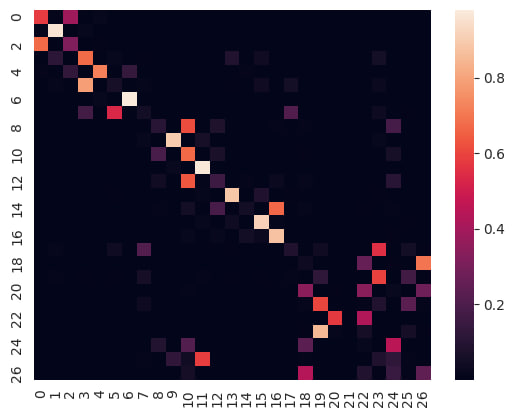
\includegraphics[width=0.5\linewidth]{figures/pairwise-cluster-heatmap.jpg}
    \caption{All similarities between contexts and responses within a dialogue. It is easy to see, that consecutive utterances form clusters.}
    \label{fig:pairwise-clister-heatmap}
\end{figure}

As a result, the obtained model is capable of recognizing individual stages in dialogues (fig. \ref{fig:pairwise-clister-heatmap}). This behavior is achieved due to two factors. Firstly, when a dialogue furthers to a new topic, the similarity between two consecutive utterances drops substantially. This is clearly visible, for example, in dialogues in which ordering a taxi replaces booking a table in a restaurant. Secondly, within one topic, there are also small drops in similarity in cases where there is a transition from one question to another. For example, the question “how many people should I book for?” replaces the question “which restaurant do you prefer?”. Moreover, since these questions relate to one topic, they remain close to themselves and distant to questions on other topics. Therefore, clusters are obtained.

(!provide the dialogue and change pic to vector instead of raster!)

\subsection{Listwise Model}

We trained the special model to merge utterances of two different dialogues (fig. \ref{fig:listwise}). It is a transformer over text embeddings of the utterances. Sentence encoder is \texttt{sentence-transformers/all-mpnet-base-v2} from hugging face. We used 4-layer transformer with 4 attention heads and hidden dimension twice smaller than sentence encoder's one, i.e. 384. Only 3 last layers of sentence encoder were fine-tuned in order to decrease computational costs.

Output ranks are transformed with softmax function. Then KL-divergence between output and target probabilities are minimized. Target probabilities are defined as softmax over true ranks of utterances, i.e. $-i$ for $i$-th utterance in dialogue.

Resulting model trains to "sort" given utterances. Thanks to the attention mechanism of transformers, this can be viewed as asking the children at physical education class to look at each other and line up by height.

To measure the sorting quality, we need to utilize appropriate metric. All traditional ranking metrics such as nDCG are designed to compare with gold ranks, not just sorting quality. So during validation of our model, we were converting the ranks to a permutation over the original sequence of $n$ elements. Then, we calculated the number of transpositions. It is easy to implement and can normalized by maximum possible number of transpositions $n(n-1)/2$, resulting in $[0,1]$-ranged metric. Our trained model reaches $0.96$ value.

\section{Composition of Augmentations}

In order to maximize diversity of training data, we use not only 5 basic augmentations described in section \ref{sec:aug}, but also 4 extra compositions of augmentations. All the resulting pipelines are defined in fig. \ref{fig:aug-compositions}. 

\begin{figure}[!htb]
    \centering
    \begin{subfigure}[t]{0.5\linewidth}
        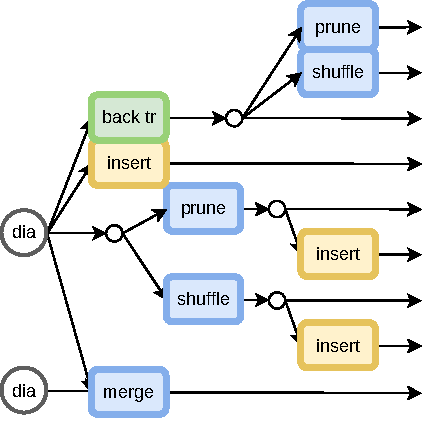
\includegraphics[width=0.85\linewidth]{figures/augmentation-pipeline-positive.drawio.pdf}
        \caption{intent-preserving}
        \centering
    \end{subfigure}
    \begin{subfigure}[t]{0.35\linewidth}
        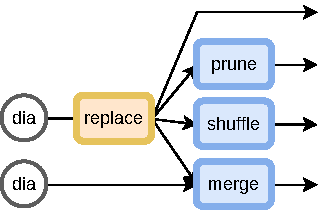
\includegraphics[width=0.9\linewidth]{figures/augmentation-pipeline-negative.drawio.pdf}
        \caption{intent-corrupting}
        \centering
    \end{subfigure}
    \caption{Compositions of augmentations.}
    \label{fig:aug-compositions}
\end{figure}

\end{document}
